\subsection{Power-to-Gas}
\label{PowertoGas_Christian}
\cfoot{Christian Geier}
\begin{parcolumns}[colwidths={1=2.5 cm, 2=10 cm, 3=2.5 cm}]{3}

\colchunk{
\textbf{Heading}
\\ 
\textbf{Introduction \\ Power-to-gas}
\\ \\ \\ \\ \\ \\ \\ \\ \\ \\
\textbf{Findings}
\\ \\ \\ \\ \\ \\ \\ \\ \\ \\ \\ \\	\\
\textit{Hydrogen use scenarios}
	 \\ \\ \\ \\ \\ \\ \\ \\ \\ \\ \\ \\
\textbf{Cost}		
\\ \\ \\ \\ \\ \\ \\ \\ \\
\textit{Alkaline investment} \\ \\ \\ 
\textit{PEM investment} \\ \\ \\ \\ \\ \\
\textit{High-Temperature investment} \\
\\ \\ 
\textit{Estimates} \\ \\ \\ \\ \\ \\ \\ \\ \\ \\ \\ \\ \\ \\ \\ \\ \\ \\ \\ \\ \\ \\ \\ \\ \\ \\ \\ \\
\textit{Prices for scenarios}  \\ \\ \\ \\ \\ \\ \\ \\
\\ \\ \\ \\ \\  \\ \\ \\ \\ \\ \\ 
\textbf{Efficiency}
\\ \\ \\ \\ \\ \\ \\ \\ \\ \\ \\ \\ \\ \\ \\  \\ \\ \\
\textit{Alkaline efficiency} \\ \\ \\
\\ \\ \\ \textit{PEM efficiency} \\ \\ \\ \\ \\ \\ \\ \\ \\ \\ \\ \\
\textbf{Safety}
\\ \\ \\ \\ \\ \\ \\ \\ \\ \\ \\ \\ \\ \\ \\ \\ 
\textbf{Scalability}
\\ \\ \\ \\ \\ \\ \\ \\ \\ \\ \\ \\ \\ \\ \\ \\
\textbf{Sustainability}
\\ \\ \\ \\ \\ \\ \\ \\ \\ \\ \\ \\ \\ \\ \\ \\ \\ \\ \\ \\
\\ \\ \\  \\ \\ \\ \\ \\ \\ 
\textbf{Technical feasibility}
\\ \\ \\ \\ \\ \\ \\ \\ \\ \\ \\ \\ \\ \\ 
\textbf{Problems and Solutions}
\\ \\ \\ \\ \\ \\ \\ \\ \\ \\ \\ \\ \\ \\ \\ \\ \\ \\ \\ \\ \\ \\
\\ \\ \\ \\ \\ \\ \\ \\ \\ \\ \\ \\ \\ 
\textbf{Conclusion}
}

\colchunk{
\\ 
Wind power plant power production is volatile and weather-dependent which leads to fluctuation, because of this, wind power is incapable of providing reliable base load power. To enable the transition to this renewable energy source, large-scale energy storage systems are required to compensate for seasonal imbalances and to save excess power. That can be achieved by converting electrical energy into hydrogen via electrolysis, a process that is called "power to gas". Water gets split into hydrogen and oxygen with the use of electricity. Hydrogen can optionally be converted to methane.
\\ \\
The paper focuses on the restricted energy that comes from wind power plants. It presents the costs, efficiency, safety, scalability, sustainabality and technical feasibility of a Power-to-Gas system. In the first 3 months of 2019 about 3.23 billion kilowatthours (kWh) had to be restricted from wind power plants. This amount is now calculated into a power by dividing the time in hours (2190h). The power now results to 1.495 million kW. This value will be used as basis for upcoming calculations. The technology of Power-to-Gas is now used as a kind of "storage" to safe the excess energy from wind power plants. There are currently three alternative concepts for Power-to-Gas systems which all use the method of water electrolysis:
\begin{itemize}
\item
Use of hydrogen from wind power for applications which require hydrogen. For example transportation or industrial applications.
\item
Direct feed-in of hydrogen from wind power into the gas grid.
\item
Methanation of the produced hydrogen with carbondioxide and feed-in of the methane into the gas grid.
\end{itemize}
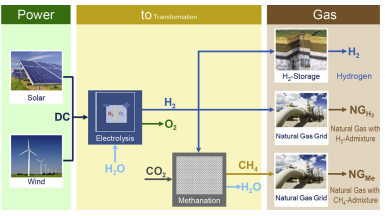
\includegraphics[scale=0.75]{schaubild}
\\
Figure 1: Concepts of power-to-gas systems. \\
Power-to-gas transforms electric energy into hydrogen which is used as energy source. So electric energy is technically not stored but transformed into a gas and can then be stored.
\\ \\
The overview for a power-to-gas energy storage in terms of cost will include investment, maintenance and operating costs. Criteria values can be seen in the outline.
\\
\textbf{Investment costs}
\\
Investment costs for a Power-to-Gas system vary greatly on the method that is used for electrolysis. Among these are alkaline water electrolysis with a liquid alkaline electrolyte, Proton Exchange Membrane (PEM) electrolysis, and High-temperature electrolysis with a solid oxide electrolyte.
\\
For alkaline water electrolysis investment costs of large-scale electrolyzers are estimated to be in the range of 800 \euro /kW to 1,500 \euro /kW. The cost of alkaline electrolyzers is very size dependent.
\\
PEM electrolyzers are a relativly new method of electrolysis and have issues related to the costs. PEM electrolyzers depend on expensive materials and result in a high investment cost of about 2,000 \euro /kW to 6,000 \euro /kW. But there is a cost reduction potential by utilizing alternative materials in the futre.
\\
High-temperature water electrolysis with a solid oxide cell is still in the stage of basic research. More investigation in materials and other characteristics is needed before a reliable value for investment cost can be given.
\\
For a simple investment estimate a constant input of 1.495 million kW is assumed (see topic \textit{Analysis}). This ignores any peaks and lows that wind power plants have. An alkaline electrolyzer is used with an average investment cost of 1,150 \euro /kW. Also, a basic efficiency of 0.7 will be included. This leads to a investment of 2.46 billion \euro{ }for electrolyzers. \\
If the produced hydrogen is feed-in into the natural gas grid investment costs are much lower, because gas (as energy source) infrastructure is already well developed in Germany. So a total investment of 2.46 billion \euro{ } in electrolyzers is needed.  \\
Also, if the methanation process is included after hydrogen is produced, investment costs increase from 2.46 billion \euro{ } to 3.075 billion \euro{ } because of lower efficiencies. This does not include additional investment costs for methanation facilities.
\\
\textbf{Maintenance and operating costs}
\\
The maintenance costs are difficult to determine for Power-to-Gas systems because the technology is still in research phase. Therefore, maintenance costs will be set to 5\% of investment costs and include the cost of replacing electrolyzers. Also, even though the power is excess power, it is not free of charge and must be paid for (0.09 \euro /kWh). In addition, a grid charge (0.02 \euro /kWh) is included and investment costs. Investment costs will be calculated based on facility lifetime (75,000h). The investment into infrastructure will be set to 1 billion \euro . The efficiency for electrolysis is set to 0.7 and for methanation to 0.8.
\\
For the first scenario, where hydrogen is feed-in into hydrogen-infrastructure for utilization (Transportation/Industry), the costs of investment would result into 0.03 \euro /kWh. Maintenance costs would be about 0.017 \euro /kWh and operating costs would be around 0.13 \euro /kWh. In this scenario a grid charge is unnecessary. The complete cost for this scenario would be about 0.177 \euro /kWh.
\\
The second scenario, where hydrogen gets a direct feed-in into the gas grid, the operating costs would be around 0.16 \euro /kWh and maintenance costs are rougly the same. The costs for investment will be set to 0.02 \euro /kWh, because additional investments in infrastructure is not needed. The complete cost sums up to 0.20 \euro /kWh.
\\
In the last scenario, where methane is synthesized, the operating costs are about 0.20 \euro /kWh because of lower efficiencies and additional feedstock costs. The investment costs also increase to 0.035 \euro /kWh. Maintenance costs are slightly higher too, but will be set as the same as in the first scenario. The sum of total costs equals to 0.252 \euro /kWh.\\
 \\
The efficiency of Power-to-Gas depends on electrolysis. The water splitting reaction is endothermic and therefore requires energy. A fraction of the energy that is put in gets lost as heat. Because of the direct injection of created hydrogen there are no real long-term storage losses. As mentioned in the section \textit{costs} there are three different electrolysis methods and all have a different efficiency. The High-Temperature solid oxide electrolysis is still on a very low technological readiness level and will be excluded, because there may be technological innovations which could increase efficiency significantly. The formula for the energetic efficiency is: \\
\begin{math}
\eta = \frac{E_{use}}{E_{input}} = \frac{E_{hydrogen}}{E_{el}} = \frac{V_{H2}* H_{s}}{U*I*t}. \\
\end{math}
V: volume of created hydrogen in cubic meter\\
H: energy volume of hydrogen in Joule/cubic meter\\
U: voltage in Volt\\
I: current in Ampere\\
t: time in hours. 
\\
The alkaline water electrolysis is available on large and small scales, with lifespans of about 10 years. The efficiency of the hydrogen production is 67\%. Assuming all excess wind power energy in Germany would be put in Power-to-Gas systems, a value of 9.17 billion kWh would result for a duration of one year. This means 3.75 billion kWh would be lost. 
\\
The Proton Exchange Membrane electrolysis is only availabe on a small scale, with lifetimes of less than 10 years. It is still a young technology, so the efficiency could be improved in the future. The efficiency in a PEM electrolysis is higher than in an alkaline water electrolysis, because of higher temperatures inside the PEM electrolysis the waste heat can be redirected to make steam and create a higher overall efficiency. This results into efficiencies of about 80\%. On the same assumption as in the alkaline water electrolysis, a value of 10.05 billion kWh would result. This leads to a loss of 2.87 billion kWh. 
\\ \\
Power-to-Gas is a reliable and safe method for transforming electrical energy into hydrogen. The only real safety threats are high hydrogenconcentrations in gas grids and oxyhydrogen reactions while electrolyzing water. High hydrogenconcentrations can damage gas pipelines, compressors and other steel components that are in contact with hydrogen. This is because of hydrogen embrittlement, which makes material fatigue happen much faster. To prevent damage the gases have to stay very pure. Gas crossover takes places in every electrolyzer, but if oxygen occurs at the cathode, where hydrogen is produced, a spontaneous combustion can happen if the mixture reaches a oxygen content of over 4 vol\% . So, the maximum value of oxygen in hydrogen is set to 2 vol\% . If this is respected, a safe operation of Power-to-Gas systems is guaranteed.
\\ \\
The scale of the Power-to-Gas facility depends on the size of the wind farm and on economic aspects. Generally the size of the electrolyzer is the most important component that has to be adjusted for a given amount of excess wind energy. \\
This is made possible through stacking single-cells and connecting them in a series. A issue with alkaline electrolyzers is that electrolyzers have a limited part-load capability of 20-40\%. Single electrolyzers have a power range from 5 kW up to 3400 kW. Multiple electrolyzers can be used in parallel operation. 
\\
PEM electrolyzers in comparision with alkaline electrolyzers have some advantages like a lower limited part-load capability of 0-10\% and slightly higher efficiencies but also have lower lifetimes. Currently, single electrolyzerers have a power range up to 150 kW. 
\\ \\
In order to rate the sustainability through water and carbon dioxide consumption, all that is needed are the respective chemical reactions. The chemical equation for a water electrolysis: \\
\[\ce{2 H2O_{(l)}  ->[\text{electrolysis}] 2 H2_{(g)} + O2_{(g)}}\]
The amount of hydrogen that is needed can be calculated through the energetic efficiency and stoichiometry.
If a hydrogen production of 2 kg is assumed and the molar masses are respected: \\
\ce{H2O} : 18 g/mol \\
\ce{O2} : 32 g/mol \\
\ce{H2} : 2 g/mol \\
a calculation is possible with \[ n = \dfrac{m}{M} \] The chemical equation tells that 2 mol of water is needed to receive 2 mol of hydrogen and 1 mol of oxygen. This leads to:
\[ 1000 \, mol \, \ce{H2O} -> 1000 \,  mol \,  \ce{H2} + 0.5*1000 \, mol \, \ce{O2} \]
Therefore, we need 18 kg of water to produce 2 kg of hydrogen. Because of efficiency a mass of 25.72 kg is needed. \\
For the optional step of methanation the amount of carbon dioxide can be calculated through stoichiometry too.
The chemical equation for hydrogen methanation :
\[\ce{CO2_{(g)} +  4 H2_{(g)} <->[\text{methanation}]  CH4_{(g)} + 2 H2O_{(g)}}\] 
The 2 kg of hydrogen that have been produced are used to produce methane. The math is the same as in the electrolysis step and will be excluded. \\
For the synthesis of 4 kg methane, a mass of 11 kg carbon dioxide and 2 kg hydrogen is needed. Because of efficiency a mass of 13.75 kg carbon dioxide and 2.5 kg hydrogen is needed.
\\ \\
The technical feasibility for Power-to-Gas depends on the use. Because of the diverse use of hydrogen there are various ways to utilize the technology. Hydrogen can be used for heating, as energy carrier and as a fuel. Right now the best use for hydrogen is using it as a fuel for transportation and industry because these are the most profitable ways to use the technology. \\
The most important technical aspect is electrolysis. In general, alkaline water electrolysis is the most developed method for Power-to-Gas systems and is ready to be used. PEM electrolysis is also in a technical feasible state, but in comparision to alkaline water electrolysis in a much more undeveloped state. High-Temperature electrolysis with a solid oxide electrolyte is currently not technically feasible. 
\\ \\ 
Power-to-Gas has currently the biggest issues related to its cost. There are also some minor issues with scalability. The problems in terms of cost are: \\ 
1. How produced hydrogen is used as a energy carrier. \\
2. The electrolyzers that are used for hydrogen production. \\
Depending on the use of produced hydrogen, a lot of investments are needed to get full use out of hydrogen. For example, if hydrogen is used as a fuel for traffic or industry, investments for electrolyzers, pipeline grids, geological storages and refueling stations are needed.
If investments into infrastructure and peak loads are taken into account, a investment cost of 86-102 billion \euro{ } is estimated by scientists. 
For the optional methanation step scientist estimate a value of 76 billion \euro{ } as investment costs.
This makes Power-to-Gas a very expensive technology to implement.\\
The only way to reduce these immense investment costs are currently just up to commercialising and research into other electrolyzing methods. Right now PEM and High-Temperature electrolysis have still potential to reach a better \euro{ } per kilowatt ratio, because these methods are still very young and new innovations could reduce costs. For alkaline electrolysis the cost per kilowatt probably will not change significantly in the future, but currently is the cheapest electrolysis method (see section \textit{Alkaline investment}).\\
The problems for scalability are the geographical and political conditions that come with wind power plants.\\
Overall Power-to-Gas is a scalable technology, but in regards of using wind power there are limitations. Wind power plants are restricted to areas with high wind velocities and few settlements. To reach a maximal supply of excess wind power, a Power-to-Gas facility needs to be close to a wind power plant. Therefore the conditions that count for wind power plants also count for a Power-to-Gas facility and need to be respected before a wind power plant and a Power-to-Gas facility can be build.\\ \\
The conclusion will look into if a Power-to-Gas system is reasonable to implement with a budget of 15 billion \euro{ } and in a span of about 10 years.\\
None of the mentioned scenarios (see section \textit{Findings}) are economical feasible (see section \textit{Maintenance and operating cost}) with this budget. For comparison the market prices for electrical power are about 0.04 \euro /kWh. The capacity that is needed during 10 years, with a constant use of 1.495 million kW, would result to 130.96 billion kWh. The costs in 10 years would be... \\
... for the first scenario ~ 23 billion \euro .\\
... for the second scenario ~ 26.2 billion \euro .\\
... for the last scenario ~ 33 billion \euro . \\
This assumes a alkaline water electrolysis because it is currently the cheapest and most reliable method to use (see section \textit{Technical feasibility} ) for a Power-to-Gas system in this time range, but in the future may be substituted with one of the two other electrolysis methods.
If the technology would be used right now, it would not be reasonable. Power-to-Gas in its current state is uneconomic, because of high investment costs, electricity prices and expensive electrolyzers. Despite this, it may become a viable method for any electrical power input in the future, since it is easy scalable for a given amount of excess power and hydrogen has diverse uses. Scientific researches show that commercialization and lower prices for power can make Power-to-Gas a reasonable application in the next 15 to 20 years.
}

\colchunk{ \textbf{References}
\begin{tiny}
\\
https://en.wikipedia.org/\\wiki/Wind\_power
\\ \\ \\ \\
https://en.wikipedia.org/\\wiki/Power-to-gas
\\ \\ \\ \\ \\ \\ \\
https://www.bdew.de/\\presse/presseinformationen\\/zahl-der-woche-gut-32-mrd-kilowattstunden/
\\ \\ \\ \\ \\ \\ \\
https://www.journals.else\\vier.com/international-journal-of-hydrogen-energy
\\ \\ \\ \\ \\ \\ \\ \\ \\ \\ \\ \\ \\ \\ \\
https://www.dena.de
\\ \\ \\
https://www.sciencedirect\\.com/science/article/pii/S\\0306261918315319
\\ \\ \\ \\ \\ \\ \\ \\ \\ \\
\\ \\ \\ \\ \\ \\ \\ \\ \\ \\ \\ \\ \\ \\ \\ \\ \\ \\ \\ \\ \\ \\ \\ \\ \\ \\ \\ \\ \\ \\ \\ \\ \\ \\ \\ \\ \\ \\ \\ \\ \\ \\ \\ \\ \\
\\ \\ \\ \\ \\ \\
https://en.wikipedia.org/\\wiki/Power-to-gas\#Efficiency
\\ \\ \\ \\ 
https://www.journals.else\\vier.com/international-journal-of-hydrogen-energy
\\ \\ \\ \\ \\ \\ \\ \\ \\ 
https://www.sciencedirect\\.com/topics/engineering/\\alkaline-water\\-electrolysis
\\ \\ \\
https://en.wikipedia.org/\\wiki/Polymer\_ electrolyte\_ membrane\_ electrolysis\# PEM\_ Efficiency
\\ \\ \\ \\ \\ \\ \\ \\
https://www.oxfordenergy.org\\/wpcms/wp-content/uploads\\/2018/10/Power-to-Gas-Linking-Electricity-and-Gas-in-a-Decarbonising-World-Insight-39.pdf
\\ \\ \\ \\ \\ 
\\ \\ \\ \\ \\
https://de.wikipedia.org/\\wiki/Power-to-Gas\# Wasserstoff\\einspeisung\_ versus\_ Methanisierung
\\ \\ \\ 
http://epub.sub.uni-hamburg.de/epub/volltexte\\/2014/35363/pdf\\/Masterthesis\_Bastian\_Hey \\
\_Power\_to\_Gas.pdf
\\ \\ \\ \\ \\ \\ \\ \\ 
https://en.wikipedia.org/\\wiki/Electrolysis\_of\_water \\ 
\#Equations
\\ \\ \\ \\ \\ \\ \\ \\ \\ \\ \\ \\ \\ \\ \\
https://en.wikipedia.org/\\wiki/Sabatier\_reaction
\\ \\ \\ \\ \\ \\ \\ \\
https://www.oxfordenergy.org\\/wpcms/wp-content/uploads\\/2018/10/Power-to-Gas-Linking-Electricity-and-Gas-in-a-Decarbonising-World-Insight-39.pdf
\\ \\ \\ \\
https://www.sciencedirect\\.com/science/article/abs/pii/\\S0360319915001913
\\ \\ \\
https://www.sciencedirect\\.com/science/article/pii/\\S0360319912026481
\\ \\ \\ \\ \\ \\ \\ \\ \\ \\ \\ \\ \\ \\ \\ \\ \\ \\ \\ \\ \\ \\ \\ \\ \\ \\ \\ \\ \\ \\ \\ \\ \\ \\ \\ \\ \\ \\ \\ \\ \\ \\ \\ \\ \\ \\ \\ \\ \\ \\ \\
https://www.sciencedirect\\.com/science/article/pii/\\S0196890415004343
\\ \\ 
https://www.sciencedirect.\\com/science/article/pii/\\S2352152X15300311
\end{tiny}
}

\end{parcolumns}
\clearpage
\cfoot{}